\chapter{Supersymmetry and the MSSM}\label{ch:supersymmetry}

Historically, examining nature at increasing energy scales (and correspondingly decreasing length scales ) has consistently yielded new physics. For example, higher-energy experiments were able to probe the structure of the weak interactions, precisely at the energy scale that the 4-Fermi theory started to fail. Similarly, the challenges listed at the end of \autoref{ch:sm} most likely point to new physics at higher energy scales, between the currently explored weak scale to the reduced Planck scale:
\begin{equation*}
M_P = 1/\sqrt{8\pi G} \approx 2.4\times 10^{18} \text{ GeV}
\end{equation*}
However, the SM Higgs potential is extremely sensitive to new physics at high energies. The mass of the SM Higgs boson receives large quantum corrections from any new physics at high energies that couples to the Higgs sector. For example, if the Higgs couples to a heavy fermion \emph{f} through a term of the form $-\lambda_fH\bar{f}f$, the one-loop correction to the higgs mass (\autoref{fig:one_loop_fermion}) takes the form
\begin{equation}
\Delta m_H^2 = -\frac{|\lambda_f|^2}{8\pi^2}\Lambda_\text{UV}^2 + ...
\label{eq:one_loop_fermion}
\end{equation}
\begin{marginfigure}
\feynmandiagram [layered layout, horizontal=b to c] { 
  a [particle=\(h\)] -- [scalar] b -- [fermion, half left, edge label=\(f\)] c -- [fermion, half left] b, c -- [scalar] d,
};
\caption{Feynman diagram for the one-loop fermionic correction to the SM Higgs mass}
\label{fig:one_loop_fermion}
\end{marginfigure}
where $\Lambda_{UV}$ is some cutoff momentum where the effects of the new physics are expected to manifest themselves. Similarly, the one-loop correction from a heavy scalar \emph{S} through the term $-\lambda_S|H|^2|S|^2$ (\autoref{fig:one_loop_scalar}) takes the form
\begin{equation}
  \Delta m_H^2 = \frac{\lambda_S}{16\pi^2}\left[\Lambda_\text{UV}^2 + ...\right]
\label{eq:one_loop_scalar}
\end{equation}
\begin{marginfigure}
\begin{tikzpicture}
\begin{feynman}
  \vertex (a){\(h\)};
	\vertex [right=of a] (b);
	\vertex [right=of b] (c);
    \vertex [above=of b] (d);
\diagram*{
	{
      [edges = scalar]
      (a) -- (b) -- (c),
      (b) -- [half left, edge label=\(S\)] (d) -- [half left] (b),
    },
};
\end{feynman}
\end{tikzpicture}
\caption{Feynman diagram for the one-loop scalar correction to the SM Higgs mass}
\label{fig:one_loop_scalar}
\end{marginfigure}
\strictpagecheck
In both these cases, the size of the correction scales quadratically with the momentum cutoff $\Lambda_{UV}$. Higher-order loop corrections can be shown to be similarly large as well. Thus the `natural' mass of the Higgs would seem to be on the the order of $\Lambda_{UV}$, which could even be as high as the Planck scale. In contrast, the actual mass that we measure is only about 126 GeV. Thus there is a \emph{hierarchy} between the observed and the `natural' mass of the SM Higgs, one of many orders of magnitude. \footnote{Note that even though only the mass of the SM Higgs is directly sensitive to $\Lambda_{UV}$, this sensitivity is propagated to all the other SM particles through their couplings to the SM Higgs.}
Thus it would seem that any UV completion of the SM would have to come with a host of parameters to tune the counterterms enough to cancel out the quadratic divergences and result in the physical mass we observe experimentally. If the new physics is at the Planck scale, the divergences must cancel to less than one part in $10^{-16}$ to give us a SM Higgs at the weak scale.
It is obviously undesirable to have to manually tune a large number of parameters to be able to come up with UV completions of the Standard Model - it would be analogous to the geocentric Ptolemaians adding an ever-increasing number of epicycles to explain what would ultimately be more simply and accurately described by Copernicus's heliocentric theory. 
Looking at the forms of the one-loop corrections in \eqref{eq:one_loop_fermion} and \eqref{eq:one_loop_scalar}, we can see that the contribution from the fermion \emph{f} will be exactly canceled out by the contributions from two complex scalars \footnote{Thus matching the number of fermionic and scalar degrees of freedom.} with $\lambda_S = |\lambda_f|^2$, the corrections from the scalar and the fermion will cancel out exactly. This suggests that the simplest way to ensure that all quadratic divergences from new physics at high energy scales cancel out is to require some kind of symmetry between fermions and scalars, ensuring that there is a scalar partner for each fermion, or vice versa.

This symmetry is known as \emph{supersymmetry}. It is a rich mathematical structure with far-reaching consequences, a lot of which are beyond the scope of this work. For a pedagogical review of supersymmetry, we refer the reader to \citep{Martin1997}. This section provides a necessarily condensed version of the treatment there. Although the hierarchy problem has been the main driving force behind the development of supersymmetry, there are other benefits that can be obtained, such as gauge coupling unification and a stable dark matter candidate, that we shall revisit in future sections.

The term `supersymmetry' refers to the invariance of the Lagrangian under supersymmetry transformations of the form
\begin{align*}
  Q|\text{Boson}\rangle = |\text{Fermion}\rangle &&\text{and}&& Q|\text{Fermion}\rangle = |\text{Boson}\rangle.
\end{align*}

Another motivation for the MSSM is that it has the right particle content to unify the strong and electroweak couplings at a high energy scale, as seen in \autoref{fig:gauge_coupling_unification}.

\begin{marginfigure}[-4cm]
    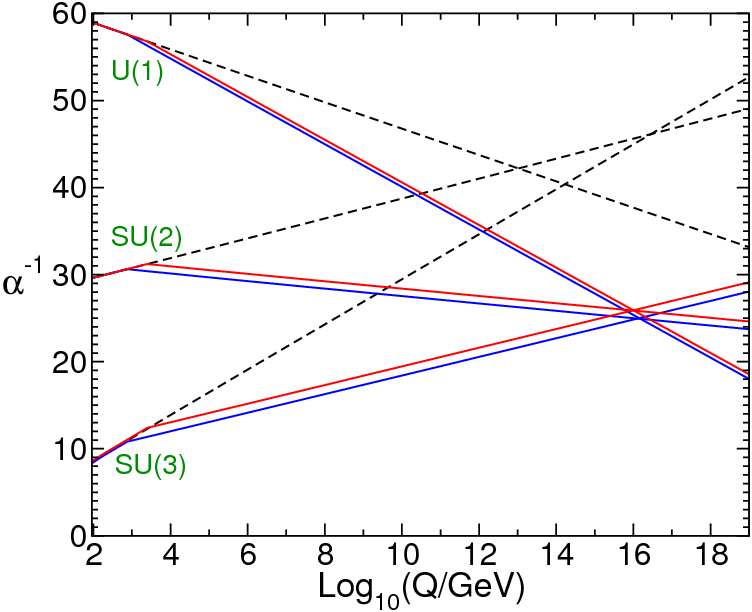
\includegraphics[width=\textwidth]{images/gauge_coupling_unification}
  \caption{2-loop RG evolution of inverse gauge couplings in the SM (dashed lines) and the MSSM (solid lines). The sparticle masses are varied between 0.5-1.5 TeV, and $\alpha_3(m_Z)$ is varied between 0.117 and 0.121. Source: \citep{Martin1997}.}
  \label{fig:gauge_coupling_unification}
\end{marginfigure}

The third major motivation (and the one most relevant to this dissertation) is the fact that the MSSM results in a viable dark matter candidate. The MSSM has a new kind of symmetry known as \emph{R-parity}. It is an analogue of baryon and lepton number conservation. The Lagrangian of the MSSM is defined to be invariant under the action of the operator $P_R$ on the fields. The eigenvalues of this operator are $(-1)^{3(B-L)+2s}$, where \emph{B, L}, and \emph{s} represent the baryon number, lepton number, and spin of the particle, respectively. The consequence of this is that the lightest supersymmetric particle (LSP) must be absolutely stable, that is, it cannot decay further into other particles, thus making it a good candidate for particle dark matter.

The minimal phenomenologically viable incorporation of supersymmetry into the Standard Model is known as the \emph{Minimal Supersymmetric Standard Model}, or the MSSM. However, before describing the salient features of the MSSM, we will outline the construction of a general supersymmetric Lagrangian with all the necessary ingredients we need: kinetic terms, mass terms, scalar self-interactions, gauge symmetry, and Yukawa interactions.

\section{Construction of supersymmetric Lagrangians}
%Symmetries of the S-matrix
In 1967, Coleman and Mandula \citep{Coleman1967} showed that, given certain assumptions, the only possible Lie group symmetries allowed for relativistic interacting field theories in four dimensions are direct products of the Poincar\'e group and an internal symmetry group (i.e. a gauge symmetry) \citep{Mandula2015}.
A Lie algebra is defined by the commutation relations of its generators. If we extend the notion of a Lie algebra to include \emph{anticommutation} relations \citep{Wess1992}, the theorem no longer applies. These kinds of algebras are known as \emph{graded Lie algebras}, or \emph{superalgebras}. The trio of Haag, Łopuszanski, and Sohnius \citep{Haag1975} applied a similar treatment as Coleman and Mandula to determine the most general superalgebra consistent with relativistic quantum field theory. The generators $Q_\alpha$ of this algebra are known as fermionic operators, and must transform as Weyl spinors. The anticommutation (and commutation) relations take the form
\begin{align}
  \begin{split}
  \{Q_\alpha, \bar{Q}_{\dot{\beta}}\} &= 2(\sigma^\mu)_{\alpha\dot{\beta}}P^\mu\\
  \{Q_\alpha, Q_\beta\} &= \{\bar{Q}_{\dot{\alpha}}, \bar{Q}_{\dot{\beta}}\} = 0\\
  [P^\mu,Q_\alpha] &= [P^\mu,\bar{Q}_{\dot{\alpha}}] = 0
\end{split}
\label{eq:susy_algebra}
\end{align}
where $P_\mu = i\partial_\mu$ is the generator of translations. 

The first supersymmetric Lagrangian density in four-dimensions was formulated by Wess and Zumino \citep{Wess1974}. The approach taken was to define infinitesimal `supergauge' transformations for scalars and spinors that generated a closed algebraic structure. Soon afterwards, Salam and Strathdee \citep{Salam1974} created a more systematic approach to constructing these transformations, by giving them a geometric interpretation. In this section, we will outline the construction of a general supersymmetric Lagrangian using the geometric method. The exposition follows that of \citep{Zee2010} and \citep{Martin1997} closely. We make extensive use of the two-component spinor notation - for a review, please see \autoref{ch:notation}.

In the geometric approach, supersymmetric transformations can be viewed as translations in a manifold known as \emph{superspace}, which is obtained by adding the `fermionic' coordinates $\theta^\alpha$, and $\bar{\theta}^{\dot{\beta}}$. Thus, the generators of these translations are represented by
\begin{align}
  Q_\alpha &= \frac{\partial}{\partial\theta^\alpha}-i(\sigma^\mu \bar{\theta})_\alpha \partial_\mu&&\text{and}&&
  \bar{Q}_{\dot{\beta}} = \frac{\partial}{\partial\bar{\theta}^{\dot{\beta}}}-i(\sigma^\mu\bar{\theta})_{\dot{\beta}}\partial_\mu.
\label{eq:susy_operators_diff_form}
\end{align}
These transformations act on objects known as superfields, which are complex scalar fields parameterized by the coordinates $(x^\mu,\theta,\bar{\theta})$
Under an infinitesimal supersymmetry transformation, a general superfield $S(x,\theta,\bar{\theta})$ transforms as
\begin{align}
S\rightarrow S' = (1+i\xi^\alpha Q_\alpha + i\bar{\xi}_{\dot{\alpha}}\bar{Q}^{\dot{\alpha}})S
\label{eq:gen_susy_transformation}
\end{align}
To construct non-supersymmetric Lagrangians, we make use of spacetime derivatives $\partial_\mu$. For supersymmetric Lagrangians, we need an analogue that commutes with supersymmetric transformations. That is, we need an operator $D$ that satisfies the condition $DS' = (DS)'$. This condition can be achieved by defining operators known as \emph{chiral covariant derivatives}, that take the form
\begin{align}
  D_\alpha = \frac{\partial}{\partial\theta^\alpha}+i(\sigma^\mu\bar{\theta})_\alpha\partial_\mu&&\text{ and }&&
  \bar{D}_{\dot{\beta}} = -\left[\frac{\partial}{\partial\bar{\theta}^{\dot{\beta}}}+i(\theta\sigma^\mu)_{\dot{\beta}}\partial_\mu\right]
\end{align}
Using these, we can define a particular kind of superfield, known as a \emph{chiral} superfield and denoted by $\Phi$, that satisfies the constraint $\bar{D}_{\dot{\beta}}\Phi = 0$. One way to implement this constraint is to define a new variable
\[y^\mu=(x^\mu+i\theta^\alpha(\sigma^\mu)_{\alpha\dot{\alpha}}\bar{\theta}^{\dot{\alpha}}).\]
Let us now simplify our notation a bit. For the rest of this section, position four-vectors such as $x^\mu$ will denoted simply by \emph{x}. With this notation, any superfield $\Phi(y,\theta)$ that is a function of only $y$ and $\theta$ will satisfy this constraint, since $\bar{D}_{\dot{\beta}}y = 0$. We perform a Taylor expansion in powers of the variable $\theta$. Now, $\theta$ is a fermionic coordinate, and has two components: $\theta^\alpha = (\theta^1,\theta^2)$. Each of the two components is a \emph{Grassmannian} variable, satisfying the anticommutation relation $\{\theta^i,\theta^i\} = 0$. This implies that $(\theta^i)^2 = 0$. For a general superfield \emph{S}, the Taylor expansion about the fermionic coordinates $\theta,\bar{\theta}$ takes the form
\begin{align}
  \begin{split}
  S(x,\theta,\bar{\theta}) = a &+ \theta\xi + \bar{\theta}\chi^\dagger + \theta\theta b + \bar{\theta}\bar{\theta}c+\bar{\theta}\bar{\sigma}^\mu\theta v_\mu \\
  &+ \bar{\theta}\bar{\theta}\theta\eta + \theta\theta\bar{\theta}\zeta^\dagger+\theta\theta\bar{\theta}\bar{\theta}d,
\end{split}
  \label{eq:general_superfield_expansion}
\end{align}
where \emph{a,b,c} and \emph{d} are complex-valued scalar fields, $\xi,\chi,\eta$ and $\zeta$ are spinor fields, and $v_\mu$ is a vector field. 
For a chiral superfield, after the redefinitions $(a,b,\xi) = (\phi,\sqrt{2}\psi,F)$, the above expansion reduces to
\[\Phi(y,\theta) = \phi(y) + \sqrt{2}\theta\psi(y)+\theta\theta F(y)\]
We can Taylor expand once more around the bosonic coordinate \emph{x} to get
\begin{align}
  \begin{split}
  \Phi(y,\theta) &= \phi(x) + \sqrt{2}\theta\psi(x)+\theta\theta F(x)\\
  &+i\theta\sigma\bar{\theta}\partial_\mu\phi(x)-\frac{1}{2}\theta\sigma\bar{\theta}\theta\sigma^\nu\bar{\theta}\partial_\mu\partial_\nu\phi(x) + \sqrt{2}\theta i\theta\sigma\bar{\theta}\partial_\mu\psi(x)
\end{split}
  \label{eq:superfield_expansion}
\end{align}
By dimensional analysis\sidefootnote{The generator $P_\mu$, represents momentum, and has dimensions of mass. We represent this by $[P_\mu] = 1$. Thus, from the supersymmetry algebra (\eqref{eq:susy_algebra}), we have $[Q] = [\bar{Q}] = \slantfrac{1}{2}.$ From the differential forms of \emph{Q} and $\bar{Q}$ in \eqref{eq:susy_operators_diff_form}, we get $[\theta]=[\bar{\theta}]=-\slantfrac{1}{2}$. Since $[\phi] = [\theta\theta]$ and we know that $[\phi] = 1$, we can deduce that $[F]=2$. An infinitesimal supersymmetry transformation changes \emph{F} by an amount $\delta F$, which then must have the same dimensions as \emph{F}. But from the form of the infinitesimal transformation in \eqref{eq:gen_susy_transformation}, we can see that $\delta F$ must be linear in $\xi$ or $\bar{\xi}$, both of which have dimension $\slantfrac{1}{2}$, and so must be multiplied by some object with dimension $\slantfrac{5}{2}$. The only such object available to us from our expansion above is $\partial_\mu\psi$, which is in reality a left-handed Weyl spinor and so carries an undotted index. Multiplying $\partial_\mu\psi^\alpha$ by the object $(\sigma^\mu)_{\alpha\dot{\alpha}}$ allows us to contract the index $\mu$ (ensuring Lorentz invariance), as well as the undotted index $\alpha$. Out of $\xi$ and $\bar{\xi}$, only $\bar{\xi}$ can be used to contract the remaining dotted index. And thus we have, up to an overall constant, $\delta F\sim\bar{\xi}^{\dot{\alpha}}(\sigma^\mu)_{\alpha\dot{\alpha}}\partial_\mu\psi^\alpha$}%
, we see that an infinitesimal change in the field $F$, denoted $\delta F$ must take the form $\delta F\sim\bar{\xi}\sigma^\mu\partial_\mu\psi$. Thus, it is a total divergence, and $\int d^4x F$ is invariant under supersymmetric transformations. We can generalize this result. Let $[\Phi]_F$ denote the coefficient of $\theta\theta$ in the expansion of a superfield $\Phi$. Then $\delta[\Phi]_F$ is a total divergence, and the integral $\int d^4x [\Phi]_F$ is invariant under supersymmetry. The next thing to note is that products of chiral superfields are also superfields: $\Phi^n$ also satisfies the requisite conditions $\bar{D}_{\dot{\beta}}\Phi^n = 0$. So an integral of the form $\int d^4x[W(\Phi)]_F$, where $W(\Phi)$ is a holomorphic \sidefootnote{That is, complex-valued and smooth.} function of the superfield $\Phi$ should also be invariant under supersymmetry. The function $W(\Phi)$ is known as the \emph{superpotential}, and contains the information about the masses and the scalar interactions of of the theory. Now let us add the kinetic terms that make the field dynamical. These terms can be obtained by bringing $\Phi^\dagger$ into the picture, since it will contain the conjugate fields $\bar{\psi}$ necessary to construct kinetic terms such as $\bar{\psi}\bar{\sigma}^\mu\partial_\mu\psi$. A first guess at a superfield that contains both $\Phi$ and $\Phi^\dagger$ is the superfield $V = \Phi^\dagger\Phi$. This field satisfies the property $(\Phi^\dagger\Phi)^\dagger = \Phi^\dagger\Phi$. In general, any superfield $V$ that satisfies the constraint $V = V^\dagger$ is known as a vector superfield.
Recalling the Taylor expansion of $\Phi$ from \eqref{eq:superfield_expansion}, the expansion of \emph{V} in powers of the fermionic coordinates looks like
\[V = \phi^\dagger\phi + 2\bar{\theta}\bar{\psi}\theta\psi + ...\]
The highest power of fermionic coordinates that we can expand to is $\bar{\theta}\bar{\theta}\theta\theta$. Since Grassmannian variables anticommute, the only non-vanishing quadratic combination will be $\bar{\theta}^{\dot{1}}\bar{\theta}^{\dot{2}}\theta_1\theta_2$. Let us follow a similar procedure as with the chiral superfields, and denote the coefficient of $\bar{\theta}\bar{\theta}\theta\theta$ in the expansion of \emph{V} by $[V]_D$. By a dimensional analysis similar to the one performed for the chiral superfields, we can show that $\delta[V]_D$ is a total divergence, and so $\int d^4x[\Phi^\dagger\Phi]_D$ is also supersymmetric. Combining $[\Phi^\dagger\Phi]_D$with our superpotential $W(\Phi)$ from earlier gives us a general supersymmetric Lagrangian:
\begin{align*}
  \mathcal{L} = [\Phi^\dagger\Phi]_D - \left([W(\Phi)]_F + h.c.\right)
\end{align*}
If we choose the superpotential of the form $W(\Phi) = \frac{1}{2}m\Phi^2 + \frac{1}{3}g\Phi^3$ and write the Lagrangian in terms of the component fields $\phi,\psi,F$, we get
\begin{align*}
  \mathcal{L} = (\partial\phi)^\dagger(\partial\phi) + i\bar{\psi}\bar{\sigma}^\mu\partial_\mu\psi+F^\dagger F-\left(mF\phi-\frac{1}{2}m\psi\psi+gF\phi^2-g\phi\psi\psi + \text{h.c.}\right)
\end{align*}
Written like this, it is evident that the component scalar and Weyl spinor fields of a superfield have the same mass. Note that this Lagrangian does not contain any derivatives of the field $F$. This means that it is not a dynamical/propagating field. We refer to $F$ as an \emph{auxiliary} field. We can get rid of of it by `integrating' it out. This can be interpreted in two ways. The first is to perform the path integral over the variables $F$ and $F^\dagger$:
\begin{align*}
\int DFDF^\dagger e^{i\int d^4x \mathcal{L}(\phi,\phi^\dagger,\psi,F,F^\dagger)} = 
 C e^{i\int d^4x \mathcal{L}(\phi,\phi^\dagger,\psi)}
\end{align*}
where $C$ is some constant, which will cancel out in computations of Green's functions, interaction vertices, etc. The other interpretation is that we can exactly solve the Euler-Lagrange equations of motion for the field \emph{F}:
\[\frac{\partial\mathcal{L}}{\partial F}-\partial_\mu\left(\frac{\partial\mathcal{L}}{\partial(\partial_\mu F)}\right) = 0.\]
For our particular Lagrangian, we can collect the terms involving $F$:
\begin{align*}
\mathcal{L}(F) &= F^\dagger F - F(m\phi+g\phi^2) - F^\dagger(m\phi+g\phi^2)^\dagger= |F-(m\phi+g\phi^2)^\dagger|^2
\end{align*}
The Euler-Lagrange equations will be satisfied if $F = (m\phi+g\phi^2)^\dagger$. Thus, after integrating out the auxiliary fields, we get
\begin{align*}
  \mathcal{L}_\text{on-shell} = |\partial\phi|^2+ i\bar{\psi}\bar{\sigma}^\mu\partial_\mu\psi-|m\phi+g\phi^2|+\left(\frac{1}{2}m\psi\psi-g\phi\psi\psi + \text{h.c.}\right)
\end{align*}
We include the hermitian conjugate (h.c.) in the Lagrangian to make the action real.The subscript `on-shell' is an indicator that this Lagrangian is supersymmetric only when the equations of motion are satisfied, i.e. the particles are on-shell. Including the auxiliary fields explicitly in the Lagrangian ensures that the Lagrangian remains supersymmetric even off-shell. So far, we have constructed kinetic terms, mass terms, interactions terms cubic and quartic in the scalar fields $\phi$, and Yukawa terms of the form $\phi\psi\psi$, out of a chiral superfield $\Phi$ and its hermitian conjugate $\Phi^\dagger$. These can be mapped onto the analogous terms in the SM Lagrangian by choosing an appropriate form for the superpotential. The other ingredient we need in this Lagrangian is gauge symmetry, and the corresponding gauge interaction terms.
Just as we obtained the fermion field $\psi$ and the scalar field $\phi$ from the Taylor expansion of a chiral superfield, we can obtain the gauge field $A_\mu^a$ (and its corresponding superpartner $\lambda^a$) from the Taylor expansion of a vector superfield.
For a vector superfield $V(x,\theta,\theta^\dagger)$, the condition $V = V^\dagger$ is equivalent to imposing the constraints
\[a = a^*, \chi^\dagger = \xi^\dagger, c = b^*, v_\mu = v_\mu^*, \zeta^\dagger = \eta^\dagger, d = d^*\]
on the expansion in \eqref{eq:general_superfield_expansion}.
For convenience, we also define:
\begin{align*}
  \eta_\alpha = \lambda_\alpha-\frac{i}{2}(\sigma^\mu\partial_\mu\xi^\dagger)_\alpha&&\text{and}&& d = \frac{1}{2}D+\frac{1}{4}\partial_\mu\partial^\mu a.
\end{align*}
With these constraints and redefinitions, the expansion of the vector superfield takes the form 
\begin{align*}
  V(x,\theta,\theta^\dagger) =& a + \theta\xi + \bar{\theta}\bar{\xi} + \theta\theta b+\bar{\theta}\bar{\theta}b^\dagger + \bar{\theta}\bar{\sigma}^\mu\theta A_\mu + \bar{\theta}\bar{\theta}\theta\left(\lambda-\frac{i}{2}\sigma^\mu\partial_\mu\bar{\xi}\right)\\
  &+\theta\theta\bar{\theta}\left(\lambda^\dagger-\frac{i}{2}\bar{\sigma}^\mu\partial_\mu\xi\right)+\theta\theta\bar{\theta}\bar{\theta}\left(\frac{D}{2}+\frac{1}{4}\partial_\mu\partial^\mu a \right)
\end{align*}
Now let us introduce the concept of \emph{supergauge} transformations. An Abelian example of a supergauge transformation is shown below.
\[V\rightarrow V+i(\Omega^*-\Omega)\]
Here, $\Omega$ is a chiral superfield that parameterizes the transformation.
Using supergauge transformations, we can eliminate the additional auxiliary fields \emph{a,b}, and $\xi$, and write the vector superfield in the \emph{Wess-Zumino} gauge:
\[V_{\text{Wess-Zumino gauge}} = \bar{\theta}\bar{\sigma}^\mu\theta A_\mu + \bar{\theta}\bar{\theta}\theta\lambda+\theta\theta\bar{\theta}\lambda^\dagger + \frac{1}{2}\theta\theta\bar{\theta}\bar{\theta}D\]
By examination, it is evident that if we wish for the field $A_\mu$ to have dimension 1 (like the gauge bosons of the SM), then $V$ must be dimensionless. In this gauge, if $\Lambda$ has an expansion such as the one in \eqref{eq:superfield_expansion}, the vector field $A_\mu$ will transform as
\begin{equation}
A_\mu\rightarrow A_\mu + i\partial_{\mu}(-i\phi^*-i\phi) = A_\mu + \partial_\mu( \text{Re}(\phi))
\label{eq:amu_supergauge_transformation}
\end{equation}
which is simply an Abelian gauge transformation. The presence of the vector field $A_\mu$ is a first hint that interactions mediated by vector bosons involve vector superfields. The field \emph{D} is an auxiliary field, similar to \emph{F}. 
In the SM, we saw that gauge fields $A_\mu$ manifest themselves in the Lagrangian by being present in the kinetic terms (through the covariant derivative) and products of field strength tensors of the form $F^{\mu\nu}F_{\mu\nu}$, where $F_{\mu\nu} = \partial_\mu A_\nu-\partial_\nu A_\mu$.
Before defining the gauge transformation rules for superfields, recall how regular (non-super) fields transform under Abelian gauge symmetries:
\[\phi\rightarrow e^{i\epsilon(x)}\phi\]
where $\epsilon(x)$ is a parameter that is space-time dependent. In fact, $\epsilon(x)$ is simply a scalar field. The supersymmetric generalization of the above transformation for a chiral superfield $\Phi$ is:
\[\Phi\rightarrow e^{2igq\Omega}\Phi\]
where $g$ is the gauge coupling and $q$ is the charge of the field under the symmetry group. The factor of 2 is conventional (to cancel out the 2 in \eqref{eq:amu_supergauge_transformation}, as we shall see). $\Omega$ is a supergauge transformation parameter, and itself a chiral superfield.
To make the kinetic term supergauge-invariant, we modify the kinetic term we had from earlier:
\[[\Phi^\dagger\Phi]_D \rightarrow [\Phi^\dagger e^{2gqV}\Phi]_D\]
where $V$ is a vector field that transforms as in \eqref{eq:amu_supergauge_transformation}. The kinetic term we had earlier, $[\Phi^\dagger\Phi]_D$, is not invariant under supergauge transformations:
\[\Phi^\dagger\Phi\rightarrow e^{-2igq(\Omega^*-\Omega)}\Phi^\dagger\Phi\]
The extra factor can be canceled out if we modify the kinetic term as follows:
\[[\Phi^\dagger\Phi]_D\rightarrow[\Phi^\dagger e^{2gqV}\Phi]_D\]
The field strength corresponding to the vector superfield \emph{V} is
\[\mathcal{W}_\alpha=-\frac{1}{4}\bar{D}\bar{D}D_\alpha V.\]
The supergauge-invariant term in the Lagrangian constructed out of these field strengths is:
\[\frac{1}{4}[\mathcal{W}^\alpha\mathcal{W}_\alpha]_F\]
Putting these terms together\footnote{There is another possible term, which we have omitted, of the form $-2\kappa[V]_D$, which is invariant under supersymmetry and supergauge transformations. This is known as a \emph{Fayet-Iliopoulos} term, and can serve as term that breaks supersymmetry softly.}, the Lagrangian for a theory with an Abelian supergauge invariance takes the form
\begin{equation*}
  \mathcal{L} = \left[\Phi^\dagger e^{2gqV}\Phi\right]_D + \left([W(\Phi)]_F + \text{h.c.}\right) + \frac{1}{4}\left([\mathcal{W}^\alpha\mathcal{W}_\alpha]_F + \text{h.c.}\right)
\end{equation*}
To generalize this to a non-Abelian gauge theory with couplings $g_a$, generators $T^a$, and associated vector superfields $V^a$, we would do the following modifications to the kinetic term and gauge transformation:
\begin{align*}
  [\Phi^\dagger e^{2gqV}\Phi]_D&\rightarrow[\Phi^\dagger e^{2g_a\mathbf{V}}\Phi]_D\\
  \Phi&\rightarrow e^{i\textbf{Ω}}\Phi
\end{align*}
where we have defined the matrix-valued fields 
\begin{align}
  \mathbf{V} = 2g_aT^aV^a&&\text{and}&& \textbf{Ω} = 2g_aT^a\Omega^a
  \label{eq:matrix_valued_fields}
\end{align}
for brevity. In this notation, the field strength for \textbf{V} is given by the chiral superfield
\[\mathcal{W}_\alpha = -\frac{1}{2}\bar{D}\bar{D}\left(e^{-\mathbf{V}}D_\alpha e^{\mathbf{V}}\right)\]
Finally, putting together all the ingredients, we have a general Lagrangian for a renormalizable supersymmetric field theory including non-Abelian supergauge invariance:
\begin{equation*}
  \mathcal{L} = \left(\frac{1}{16k_ag_a^2}-i\frac{\Theta_a}{128k_a\pi^2}\right)\text{Tr}[\mathcal{W}^a\mathcal{W}_a]_F + \text{h.c.} + \left[\Phi^\dagger(e^{\mathbf{V}})\Phi\right]_D + \left([W(\Phi)]_F + \text{h.c.}\right)
\end{equation*}
Here, $k_a$ defines the normalization of the generators: $\text{Tr}[T^aT^b] = k_a\delta_{ab}$, and is conventionally set to $\slantfrac{1}{2}$. The parameter $\Theta$ is a CP-violating parameter similar to the angle $\theta$ discussed at the beginning of \autoref{ch:2HDMs}. The Fayet-Iliopoulos term that we saw for Abelian supergauge symmetry is no longer allowed since individual terms of the form $-2\kappa[V^a]_D$ are no longer invariant under supergauge transformations - they induce mixing among the vector fields $V^a$ (which is why we worked instead with the matrix-valued fields from \eqref{eq:matrix_valued_fields}).

\section{Chiral and gauge supermultiplets}
All the particles in the MSSM are grouped into structures known as supermultiplets. They come in two varieties: \emph{chiral} and \emph{gauge} supermultiplets. The SM fermions and the components of the SM Higgs doublet reside inchiral supermultiplets, and the SM gauge bosons reside in gauge supermultiplets. Let us first look at what the gauge interactions of a generic chiral and gauge supermultiplet look like.
For a generic chiral supermultiplet consisting of a complex scalar \emph{ϕ} and its superpartner, a two-component Weyl fermion $\psi$, the kinetic terms are 
\[\mathcal{L}_{\text{chiral,kinetic,fermion}} = -\partial^\mu\phi^*\partial_\mu\phi + i\psi^{\dagger}\overline{\sigma}^\mu\partial_\mu\psi.\]
If the Lagrangian density is invariant under gauge transformations of the chiral supermultiplet under a gauge group with generators $(T^a)_i^j$ and associated gauge fields $A_\mu^a$, the partial derivatives above can be promoted to covariant derivatives:
\begin{align}
  \nabla_\mu\phi_i &= \partial_\mu\phi_i - igA_\mu^a(T^a\phi)_i\label{eq:phi1}\\
  \nabla_\mu\phi^{*i} &= \partial_\mu\phi^{*i} + igA_\mu^a(\phi^*T^a)^{i}\label{eq:phi2}\\
  \nabla_\mu\psi_i &= \partial_\mu\psi_i - igA_\mu^a(T^a\psi)_i\label{eq:psi}
\end{align}

\subsection{Interactions}
\subsection{The superpotential}
The MSSM superpotential takes the form
\[W_\text{MSSM} = \bar{u}\mathbf{y_u}QH_u-\bar{d}\mathbf{y_d}Q H_d-\bar{e}\mathbf{y_e}L H_d+\mu H_u H_d \]

The non-SM interactions in our signal process are the higgsino-bino-$Z$ and the higgsino-bino-$h$ interactions. To determine their coupling, we can inspect the structure of the MSSM. We will first examine the gauge interactions of higgsino and bino gauge eigenstates. Upon doing this, it will be apparent that there are no interaction terms containing both pure higgsinos and pure binos. The reason is that electroweak symmetry breaking induces mixing among the neutralinos. After this, we will move on to the coupling involving the SM Higgs boson, and see how it is obtained. 
In the MSSM, there are two $SU(2)_L\times U(1)_Y$ Higgs doublets instead of the one that we encounter in the standard model.
\[H_u = \begin{pmatrix}H_u^+\\H_u^0\end{pmatrix};
H_d = \begin{pmatrix}H_d^0\\H_d^-\end{pmatrix}\]
Inserting the covariant derivatives into the kinetic terms will yield the interaction terms. Each of the fields $H_u$ and $H_d$ can be interpreted as the scalar field $\phi$ in \eqref{eq:phi1} and \eqref{eq:phi2}. Similarly, the supersymmetrizations of $H_u$ and $H_d$,
\[\widetilde{H_u} = \begin{pmatrix}\widetilde{H_u}^+\\\widetilde{H_u}^0\end{pmatrix};
\widetilde{H_d} = \begin{pmatrix}\widetilde{H_d}^0\\\widetilde{H_d}^-\end{pmatrix}\]
can be equated with the field $\psi$ in \eqref{eq:psi}. The component fields of these are called \emph{higgsinos}. Once we insert the generators and associated gauge fields for the $SU(2)_L\times U(1)_Y$ symmetry in the covariant derivatives, and mix the gauge fields in the manner dictated by electroweak symmetry breaking, the gauge interactions of the higgs and higgsino fields look a lot like the SM interactions. In fact, they will have the same strength. Since we are interested in neutral higgsino-like NLSPs for our signal process, let us isolate their particular interaction terms:
\[\frac{g}{\cos\theta_W}Z_\mu\left(\widetilde{H_u}^{0\dagger}\overline{\sigma}^\mu \widetilde{H_u}+
\widetilde{H_d}^{0\dagger}\overline{\sigma}^\mu \widetilde{H_d}\right)\]
Now let us turn to the interactions of gauge supermultiplets. A generic gauge supermultiplet will consist of a gauge boson $A_\mu^a$ and its two-component Weyl fermion superpartner, the \emph{gaugino} $\lambda^a$. The SM gauge bosons reside in such gauge supermultiplets, and so the index $a$ runs over the adjoint representation of the relevant gauge group. The gauge interactions of gauginos can be extracted from their kinetic term in the Lagrangian:
\[\mathcal{L}_{\text{gaugino,kinetic}} = i\lambda^{a\dagger}\overline{\sigma}^\mu\nabla_\mu\lambda^a\]
where the covariant derivative is given by
\[\nabla_\mu\lambda^a = \partial_\mu\lambda^a + gf^{abc}A_\mu^b\lambda^c.\]
The factors $f^{abc}$ represent the structure constants of the gauge group. Thus, the interaction term would look like:
\[ig\lambda^{a\dagger}\overline{\sigma}^\mu f^{abc}A_\mu^b\lambda^c\]
The bino $(\widetilde{B}^0)$ is the superpartner of the SM gauge boson associated with the $U(1)_Y$ (hypercharge) gauge symmetry. Thus, it will transform in the adjoint representation of $U(1)_Y$ as well. However, this implies that there can never be a interaction vertex containing a bino and a gauge boson, since the structure constants for $U(1)_Y$ are all simply 0. In addition, we have previously seen that examining the chiral supermultiplet conaining the higgsino does not yield a neutral higgsino-bino-$Z$ vertex either. The reason that we can consider such a vertex in our signal process is due to the fact that electroweak symmetry breaking induces mixing among neutral higgsinos, binos, and the neutral wino $(\widetilde{W}^0)$, the superpartner of the $W_\mu^3$ gauge field associated with the SM $SU(2)_L$ gauge symmetry that mixes with $B_\mu$ to form the $Z$ boson and photon.

\section{Split Supersymmetry}
With the tightening constraints on the MSSM from the LHC, it is worth considering what would happen if we relaxed our idea of `naturalness'. Such a spectrum is called a \emph{split} spectrum, with a hierarchy between the masses of the fermionic and scalar superpartners.
